
\section{Decentralized real-time editor}
\label{sec:editor}

% Distributed collaborative editors such as Google Docs, Etherpad, or SubEthaEdit,
% allow collaborators to work distributed in time, space, and
% organizations~\cite{ellis1991groupware}. These tools improve the implication of
% users as well as the quality of documents. However, trending editors such as
% Google Docs rely on central servers which bring issues in privacy, scalability,
% and robustness. Decentralized editors settle issues in privacy and robustness
% but scalability issues remain.

% We believe that editors should allow collaborative editing whatever the number
% of collaborators, whatever their location, whenever they need, without third
% parties.

\begin{figure}
  \centering
  \begin{tikzpicture}[scale=1.1]

\newcommand\X{25pt}
\newcommand\Y{20pt}

\newcommand\LIGHTGRAY{gray!20}

\small
%% communication
\draw[rounded corners=2mm, fill=white](0pt, 0pt)+(-4*\X,-\Y)rectangle+(4*\X,\Y);
\draw(4*\X, \Y)node[anchor=north east]{\textbf{communication}};

\draw[fill=white](-2*\X, -0.25*\Y)
node{broadcast}+(-0.75*\X,-0.5*\Y)rectangle+(0.75*\X,0.5*\Y);
\draw[fill=white, thick]( 0*\X, 0.25*\Y)
node{\SPRAY}+(-0.75*\X,-0.5*\Y)rectangle+(0.75*\X,0.5*\Y);
\draw[fill=white]( 2*\X, -0.25*\Y)
node{unicast}+(-0.75*\X,-0.5*\Y)rectangle+(0.75*\X,0.5*\Y);

\draw[<-](-0.75*\X, 0.25*\Y)--(-1.25*\X, -0.25*\Y);
\draw[<-](0.75*\X, 0.25*\Y)--(1.25*\X, -0.25*\Y);

%% causality
\draw[rounded corners=2mm, fill=\LIGHTGRAY](0pt, -2*\Y)+(-4*\X,-\Y)rectangle+(4*\X,\Y);
\draw(4*\X, -\Y)node[anchor=north east]{\textbf{causality}};

\draw[fill=\LIGHTGRAY](-2*\X, -2*\Y)
node[align=center]{version vector\\with\\exceptions}
+(-1.0*\X,-0.6*\Y)rectangle+(1.0*\X,0.6*\Y);

\draw[<->, thick](-2*\X, -0.75*\Y)--(-2*\X, -1.4*\Y);
\draw[<->]( 2*\X, -0.75*\Y)--( 1*\X, -2.5*\Y);

%% sequence structure
\draw[rounded corners=2mm, fill=white](0pt, -4*\Y)+(-4*\X,-\Y)rectangle+(4*\X,\Y);
\draw(4*\X, -3*\Y)node[anchor=north east, align=right]
{\textbf{sequence}\\\textbf{structure}};

\draw[fill=white, shading=axis,top color=\LIGHTGRAY, bottom color=white, shading angle=0](1*\X, -3*\Y)
node{anti-entropy}+(-0.95*\X,-0.5*\Y) rectangle +(0.95 *\X, 0.5*\Y);
\draw[fill=white, thick](-2*\X, -4*\Y)
node{\LSEQ}+(-0.75*\X,-0.5*\Y) rectangle +(0.75 *\X, 0.5*\Y);

\draw[->] (0.05*\X, -2.75*\Y)--(-1*\X,-2*\Y);
\draw[->] (0.05*\X, -3.25*\Y)--(-1.25*\X,-4*\Y);
\draw[<->, thick] (-2*\X, -3.5*\Y)--(-2*\X, -2.6*\Y);

%% gui
\draw[rounded corners=2mm, fill=\LIGHTGRAY](0pt, -6*\Y)+(-4*\X,-\Y)rectangle+(4*\X,\Y);
\draw(4*\X, -5*\Y)node[anchor=north east, align=right]
{\textbf{graphical}\\\textbf{user}\\\textbf{interface}};
\draw[fill=\LIGHTGRAY](0pt,-6*\Y)
node{web editor}+(-0.85*\X,-0.5*\Y) rectangle +(0.85 *\X, 0.5*\Y);

%%\draw[<->] (-2*\X, -4.5*\Y) -- (0*\X, -5.5*\Y);
\draw[<->, thick] (-2*\X, -4.5*\Y) -- (-0.85*\X, -6*\Y);
\end{tikzpicture}
  \caption{\label{fig:architecture}The four layers of decentralized editors'
    architecture.}
\end{figure}


Figure~\ref{fig:architecture} describes the decentralized editors' architecture
that comprises 4 layers where each can constitute an obstacle to scalability:
\begin{inparaenum}[(i)]
\item the communication layer includes the editing session membership mechanism
  and the information dissemination protocols;
\item the causality layer includes the causality tracking structure and the
  catch up mechanism; %that
%  guarantees a delivery order of operations reflecting a form of causality,
%  e.g. it ensures that the removal of an element always follows its insertion;
\item the sequence layer includes a convergent replicated structure representing
  the document;
\item the user interface layer includes the editor as a graphical entity that
  users can interact with. %% inside web browsers.
\end{inparaenum}

The left part of the figure depicts the common process chain: when a user
performs an operation on the document, the operation is applied to the
distributed sequence. Then it decorates the operation with causality tracking
metadata. Finally, the editor broadcasts it using the neighborhood provided by
the membership protocol.  Conversely, when the editor receives a broadcast
message, it checks if the operation is causally ready to be delivered. Once the
condition is verified, it applies the operation to the distributed sequence
which notifies the graphical user interface of the changes.  The right part of
the figure corresponds to the catch up strategy where a member may have missed
operations due to dropped messages, or simply because the user worked on offline
mode for a while. Therefore, when the editor is online, it regularly asks to its
neighborhood for the missing operations.

\CRATE~\cite{nedelec2016crate} is a real-time decentralized editor running
directly within web browsers and available at
\url{https://github.com/Chat-Wane/CRATE}. 
%% None of its internal components prevent its scalability.
This section describes the components of \CRATE present in each layer and it
reviews their contribution to the scalability of the system. Among others, the
communication complexity scales well in terms of number of participants and
document size. Section~\ref{sec:experiments} validates this claim through
experiments.
%% Other dimensions such as concurrency rate are not part of 


\subsection{Communication}
\label{subsec:communication}

Editing sessions can gather from small to large groups during their life time,
e.g., massive open online courses (MOOC) may start with a large number of
students which can quickly decrease due to a lack of
interest~\cite{breslow2013studying}. Also, editing sessions vary from their size
according to the scope of documents. For instance, a document describing a
personal project and the visibility of which is limited to friends gathers
significantly less people than a document about a large event, such as a
collaboratively written report about a conference. The communication layer
should transparently handle any editing session size in a scalable manner.

%% Among others, each member of the editing session must be able to start editing 
%% whenever she wants.

\CRATE uses \SPRAY~\cite{nedelec2015spray} to automatically adapt its
functioning to the editing session size. \SPRAY is a random peer sampling
protocol~\cite{jelasity2007gossip} that incrementally builds and maintains the
neighborhood of editors. Thus, each editor has a small set of editors to
communicate with. The size of sets scales logarithmically compared to the number
of current participants in the editing session. If the editing session starts
with 10 participants, they have 2.3 neighbors in average. If the editing session
grows to 1000 connected participants, they have 6.9 neighbors in average. If the
editing session shrinks to 10 participants again, they have 2.3 neighbors in
average again.

To broadcast operations, the editor makes extensive use of neighborhoods to
propagate changes. Indeed, when a user performs a change, the editor sends it to
the editors in its neighborhood. Each neighbor is in charge of integrating and
forwarding the change to its own neighbors. Changes transitively reach all
editors very quickly, for the average shortest path from an editor to others
remains very small. The communication complexity at each editor is upper-bounded
by $\mathcal{O}(M \ln(R))$, where $M$ is the message size, and $R$ is number of
replicas connected during the propagation.

%% The code of \SPRAY building networks of browsers is available at
%% \url{https://github.com/Chat-Wane/spray-wrtc}.

% To collaboratively edit a document, users must establish a form of communication
% between them. It firstly requires accessing the editing session. It secondly
% requires building a network of communication channels. It thirdly requires the
% members to use it to spread the changes performed on shared documents.  

% \subsubsection{First access}

% The first access to an editing session transits a signaling server. A member
% wishing to share the document provides a \emph{uniform resource locator} (URL)
% that contains
% \begin{inparaenum}[(i)]
% \item an address to the \CRATE's files with the web application
%   code,
% \item and a reference to the editing session. Note that the latter must be
%   unique (for the signaling server and during the sharing time) and
%   immutable (to one document corresponds one editing session).
% \end{inparaenum}
% For instance, the URL \url{http://chat-wane.github.io/CRATE?snow-crab} targets
% the Github file server, and asks to the signaling server about the editing
% session called \emph{snow-crab}.  The signaling server chooses at random an
% available contact among sharers of this editing session. After a round-trip of
% messages, the first WebRTC connection is established, i.e., a connection from
% browser-to-browser that enables real-time communication. Since the joiner has
% access to the editing session through its contact, it does not need the
% signaling server any longer, hence, it disconnects from it. The member
% establishes other WebRTC connections using a membership protocol.

% \subsubsection{Membership}

% The membership protocol, called \SPRAY~\cite{nedelec2015spray}, is a random peer
% sampling protocol~\cite{jelasity2007gossip} the primary target of which is
% WebRTC.  As such, the range of users includes small devices (e.g. smartphones,
% tablets, etc.) and establishing a connection requires a three-way
% handshake. These constraints invite to maintain a small number of connections.

% Using \SPRAY, each member owns a set of neighbors which dynamically grows and
% shrinks to reflect the network size. Without any global knowledge,
% \begin{inparaenum}[(i)]
% \item it provides each member with a neighborhood of logarithmic size compared
%   to the global network size;
% \item it quickly converges to a topology exposing similarities with random
%   graphs~\cite{erdos1959random}. Among others,
%   \begin{inparaenum}[(a)]
%   \item it balances the load among members by repeatedly averaging over time the
%     size of neighborhoods pairwise;
%   \item it becomes robust to random crashes or unexpected departures of
%     members;
%   \item the shortest average distance to reach all peers stays small.
%   \end{inparaenum}
% \end{inparaenum}

% \SPRAY divides the life-cycle of a member into three phases: the joining, the
% exchanges, and the leaving. They respectively aim to increase, to retain, and
% to decrease the number of connections following a logarithmic progression.

% \subsubsection{Broadcast}

% The information dissemination protocol\cite{birman1999bimodal} aims to propagate
% the changes performed by users on their shared document. Any operation must
% reach all members (broadcast) to guarantee eventual consistency.  When a user
% performs an operation, \CRATE prepares a message including the result of the
% operation and sends it to the whole network using its neighborhood. Neighbors
% receiving such message forward it to their own neighbors. Hence, messages reach
% all participants transitively. To guarantee termination and to limit the
% flooding, each member forwards each message to their neigbhors only once by
% using a version vector with exceptions (cf. Section~\ref{subsec:causality}).

% Compared to state-of-the-art~\cite{ganesh2003peer, jelasity2007gossip,
%   voulgaris2005cyclon}, \SPRAY provides a neigbhorhood reflecting the network
% size instead of a constant size neighborhood set at start (commonly oversized to
% handle large networks). As such, information dissemination protocol on top of
% \SPRAY adapts the load to the network size.

% The information dissemination protocol impacts the communication complexity at
% each member:
% \begin{equation}
%   \mathcal{O}(m.\ln R)
% \end{equation}
% where $m$ is the message size determined by the layers below, and
% $R$ is the number of replicas in the network including both
% writers and readers of the shared sequence.


\subsection{Causality tracking}
\label{subsec:causality}

To preserve consistent replicas, the same outcome must result from the
generation of the operation and its integration~\cite{sun1998achieving}. Often,
the behavior of an operation depends of others previously integrated. For
instance, the generation of a removal operation requires the targeted element to
exist, hence, its insert operation to be integrated. These \emph{happens before}
relationships~\cite{lamport1978time} constrain the integration order.
Unfortunately, the more the order is constrained, the costlier it
becomes. Accurately tracking causal relations of one operation with all others
requires at least $\mathcal{O}(W)$ both locally and in communication overhead,
where $W$ is the number of participants that ever wrote in the
document~\cite{charronbost1991concerning}. Such communication overhead confines
its usage to small editing sessions.

\CRATE tracks only the semantically related pairs of operations: the removal of
an element with its insertion. If the operations arrives to an editor out of
order, the removal waits for the corresponding insertion. On the opposite, it
immediately integrates received insertions. \CRATE uses a version vector with
exceptions~\cite{malkhi2007concise, mukund2014optimized}: for each editor,
\begin{inparaenum}[(i)]
\item an integer denotes the maximal counter of received operations that
  originated from this editor and
\item a set of integers denotes the exceptions, i.e., the operations known as
  not yet received from this editor.
\end{inparaenum}
For instance, in Figure~\ref{fig:timeline}, the vectors are represented as a
list of triples
$\langle unique\,site\,identifier,\, maximal\,counter,\, exceptions \rangle$.
The second editor happens to obtain the vector $[\langle u_1,\,2,\ \{1\}]$.  It
states that $u_2$ received 1 operation from $u_1$ with the counter 2 but another
operation exists -- the first one of $u_1$ -- that $u_2$ did not yet received.

While the local overhead implied by such structure remains upper-bounded by
$\mathcal{O}(W)$, the communication overhead is constant $\mathcal{O}(1)$.

%% The causality tracking structure is available at
%% \url{https://github.com/Chat-Wane/version-vector-with-exceptions}.

The structure also serves as a tool to identify differences between replicas
when an editor needs to catch up with the current state of the document in the
live editing session. The anti-entropy protocol~\cite{demers1987epidemic}
reduces the information differences between the involved members. It selects an
editor from its neighborhood at random, and sends its local version vector with
exceptions. The chosen neighbor performs the difference with its own vector,
searches the missing operations, and sends them back to the requesting
editor. All editors periodically perform such anti-entropy rounds ensuring that
no operations went missing -- due to unpredictable network behavior or because
some collaborators worked offline.

%% To guarantee the exactly once delivery of operations, and the causal delivery
%% of semantically related operations, \CRATE uses a version vector with
%% exceptions~\cite{malkhi2007concise, mukund2014optimized}.

% \subsubsection{Version vector with exceptions}

% A vector stores for each member
% \begin{inparaenum}[(i)]
% \item an integer denoting the maximum counter of operations originated from
%   this site and
% \item a list of integers denoting the exceptions, i.e., the operations known
%   as not received yet.
% \end{inparaenum}

% A unique member identifier along with a monotonically growing counter allows
% differentiating each operation. Thus, when a member performs a change to its
% shared document, it increments its local counter. Then it decorates the message
% with its counter and identifier. Upon reception, \CRATE checks in the version
% vector with exceptions if it already received the operation earlier. In this
% case, it simply discards the operation.  Otherwise, it checks if the operation
% depends on another one. In this case, \CRATE delivers the operation if this
% other operation is delivered. Otherwise, it puts the operation in a buffer
% awaiting for the dependency to arrive. Upon delivery, it integrates the
% operation identifier to the version vector with exceptions.

\begin{figure}
  \centering
  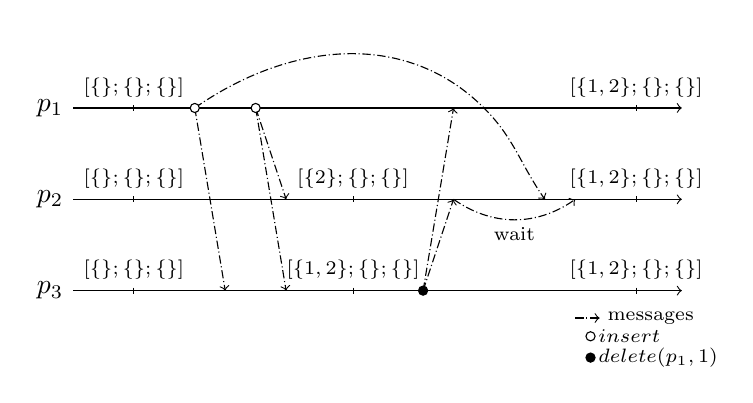
\begin{tikzpicture}[scale=1.1]
  
  \draw (-10pt,0pt) node[anchor=east]{$p_1$};
  \draw (-10pt,-30pt) node[anchor=east]{$p_2$};
  \draw (-10pt,-60pt) node[anchor=east]{$p_3$};

  \draw[->] (-10pt,0pt) -- (190pt,0pt);
  \draw[->] (-10pt,-30pt) -- (190pt,-30pt);
  \draw[->] (-10pt,-60pt) -- (190pt,-60pt);

  \scriptsize
  \draw (10pt,1pt) node[anchor=south]{[$\{\};\{\};\{\}]$} --
  (10pt,-1pt);
  \draw (10pt,-29pt) node[anchor=south]{[$\{\};\{\};\{\}]$} --
  (10pt,-31pt);
  \draw (10pt,-59pt) node[anchor=south]{[$\{\};\{\};\{\}]$} --
  (10pt,-61pt);

  \draw[->,densely dashdotted] (30pt,0pt) -- (40pt,-60pt);
  \draw[->,densely dashdotted] (50pt,0pt) -- (60pt,-30pt);
  \draw[->,densely dashdotted] (50pt,0pt) -- (60pt,-60pt);


  \draw (82pt,-29pt) node[anchor=south]{[$\{2\};\{\};\{\}]$} --
  (82pt,-31pt);
  \draw (82pt,-59pt) node[anchor=south]{[$\{1,2\};\{\};\{\}]$} --
  (82pt,-61pt);

  \draw [->,densely dashdotted] (30pt,0pt) to[out=35,in=135] (125pt,0pt)
  to[out=-45,in=125] (145pt,-30pt);

  \draw[fill=white] (30pt,0pt) circle (1.5pt);
  \draw[fill=white] (50pt,0pt) circle (1.5pt);

  \draw[->,densely dashdotted] (105pt,-60pt)--(115pt,-30pt);
  \draw[->,densely dashdotted] (105pt,-60pt)--(115pt,0pt);

  \draw[fill=black] (105pt,-60pt) circle (1.5pt);
  
  \draw[->,densely dashdotted]
  (115pt,-30pt)to[out=-35,in=-145]node[anchor=north]{wait}(155pt,-30pt);


  \draw (175pt,1pt) node[anchor=south]{$[\{1,2\};\{\};\{\}]$}-- (175pt,-1pt);
  \draw (175pt,-29pt) node[anchor=south]{$[\{1,2\};\{\};\{\}]$}--(175pt,-31pt);
  \draw (175pt,-59pt) node[anchor=south]{$[\{1,2\};\{\};\{\}]$}--(175pt,-61pt);
  
  \draw[->,densely dashdotted] (155pt,-69pt) -- (163pt,-69pt)
  node[anchor=west]{messages};
  \draw[fill=white] (160pt,-75pt)node[anchor=west]{$insert$}circle (1.5pt);
  \draw[fill=black] (160pt,-82pt)
  node[anchor=west]{$delete(p_1,1)$} circle (1.5pt);

\end{tikzpicture}

  \caption{\label{fig:timeline} Causality tracking example involving 3
    editors. The version vectors with exceptions are vectors of triples
    $\langle unique\,site\,identifier,\, maximal\,counter,\, exceptions
    \rangle$.}
\end{figure}

Figure~\ref{fig:timeline} depicts an editing session involving 3 editors. The
version vectors with exceptions start empty. The editor $u_1$ inserts two
characters in its replica and broadcasts the corresponding messages. The editor
$u_3$ quickly receives both operations. Since it did not receive these
operations before, and since they do not depend of any other operation, the
editor integrates the received counters to its vector. It also delivers the
operation to the shared sequence structure. In the meantime, the editor $u_2$
only received the second operation. Consequently, it stores this maximal
counter, marks the first operation of $u_1$ as exception, and delivers the
received operation. Then, $u_3$ removes the first character inserted by $u_1$
and broadcasts the corresponding message. While $u_1$ delivers the removal
immediately, $u_2$ waits, for the targeted operation belongs to its
exceptions. Once it receives the missing operation of $u_1$, the exception
disappears and the delete operation is delivered.

% The local upper-bound on space complexity is:
% \begin{equation}
%   \mathcal{O}(W)
% \end{equation}
% where $W$ is the number of writers, i.e., users who modified the
% document at least once.  Such structure only requires to piggyback the
% identifiers of operation. Hence, the upper-bound on communication complexity
% is:
% \begin{equation}
%   \mathcal{O}(o.\ln R|)
% \end{equation}
% where $o$ is the operation size determined by the shared sequence structure
% (cf. Section~\ref{subsec:sequence}), and the rest is determined by the
% communication layer (cf. Section~\ref{subsec:communication}).

% \subsubsection{Anti-entropy} 

% The anti-entropy protocol periodically checks if the local replica diverges from
% another neighbor's one at random. It aims to retrieve missing operations that
% could have been lost during transmissions. For this purpose, a simple difference
% between vectors suffices.

% For instance, in the prior example depicted by Figure~\ref{fig:timeline}, Member
% $m_2$ receives the second operation of $m_1$ before its first. To catch up,
% $m_2$ could send its version vector with exceptions to one of its neighbors
% chosen at random. Assuming that it picks $m_3$, the latter detects that,
% compared to its own vector, the remote member missed the first operation of
% $m_1$. Then, it sends it back to $m_2$ along with its own vector. Finally, $m_2$
% follows the normal process for the received operations, and additionnaly merges
% its vector with the received one.

% Such protocol does not require any additional local metadata. However, the
% communication cost is prohibitively high which encourages to perform this
% reconciliation protocol with great care:
% \begin{equation}
%   \mathcal{O}(W+W+x.o)
% \end{equation}
% where the first $W|$ designates the vector contained in the initiating
% message, and $W+x.o$ the response to this message where $x.o$ are the missing
% operations.

\subsection{Shared sequence}

Strong eventual consistency states that a system is correct if and only if
replicas integrating a same set of operations converge to an equivalent
state~\cite{shapiro2011comprehensive}. The shared sequence structure aims to
provide convergent copies of the document. Thus, users visualize the same
document.

\CRATE uses a conflict-free replicated data type for
sequences~\cite{shapiro2011conflict} to represent its documents. Such sequence
types rely on unique and immutable identifiers. \CRATE uses \LSEQ to provide the
identifiers. Delete operations truly remove the targeted element from the
underlying structure. Furthermore, the size of these identifiers are expected to
be bounded between a logarithmic bound and a polylogarithmic bound compared to
the number of insertions in the sequence. Being sublinear, the communication
complexity becomes acceptable. Being sublinear, the structure does not require
balancing which needs consensus algorithms that do not
scale~\cite{mostefaoui2015signature}.

%% The code of \LSEQ is available at
%% \url{https://github.com/Chat-Wane/LSEQTree}.

The logarithmic multiplicative factor of broadcast, the constant cost of
causality tracking, and the cost of identifiers, lead to a communication
complexity bounded between $\mathcal{O}((\log I).(\ln R))$ and
$\mathcal{O}((\log I)^2.(\ln R))$ depending on the editing behavior, where $I$
is the number of insert operations performed on the sequence, and $R$ the number
of replicas in the editing session during the message propagation.

\subsection{Graphical user interface}

Each participant owns a replica of the shared document. Yet the application must
give the illusion of a single document being accessed by multiple
participants.

\CRATE is a real-time editor -- written in HTML, CSS, and JavaScript -- that
runs directly within web browsers. It establishes browser-to-browser
communications using the recent WebRTC technology~\cite{webrtc}. It provides a
user friendly editor using Ace~\cite{ace}.

%% It uses the Ace code editor available at \url{https://ace.c9.io} to create
%% the view available to users.

Since CRDTs for sequences provide functions relying on identifiers rather than
indexes, \CRATE uses a lookup function which gets the identifiers at a
designated index, and conversely. Recall that the lookup time complexity is
upper-bounded by $\mathcal{O}(2^{\sqrt{\log I}})$ for random editing and by
$\mathcal{O}(I)$ for monotonic editing -- the latter being the worst case
scenario. However, as stated in Section~\ref{subsubsec:time}, it constitutes a
very pessimistic upper bound, for the efficiency of the operation can be easily
improved.

Users are always able to modify the document whenever they please.  When users
perform their insertions, \CRATE gets the identifiers at the targeted position
and generates the new identifier. When it receives an identifier, it firstly
inserts it into the tree structure and secondly get its index to notify the
view. As such, users can edit in real-time, i.e. they do not experience any
freezes during their edition locally, remote insertions are integrated as soon
as possible.

% Each element in the tree keeps track of its number of children. Such information
% allows quick withdrawing of ranges of elements. Table~\ref{table:lseqlookup}
% shows the time complexity of the look-up operation. When the tree structure is
% balanced, only a small fraction of the tree need to be browsed to find the index
% of elements. On the other hand, the structure generated by monotonic editing
% leads to a linear look-up. Fortunately, the latter case does not happen at local
% insertions since \CRATE can lazily store the last generated identifier to create
% the new one. If a user starts to edit each time at different positions, the
% structure starts to be balanced, and the look-up becomes more efficient
% relatively to the document size. Upon reception, since users only have a partial
% view of the whole document, the look-up of the received operation may fall into
% a range of element not loaded by the view.


%%% Local Variables: 
%%% mode: latex
%%% TeX-master: "../paper"
%%% End: 
